\documentclass[11pt]{amsbook}
\usepackage[turkish]{babel}

\usepackage{../Ceyhun}	% ------------------------
\usepackage{../amsTurkish}

\begin{document}
	\hPage{ceyhun-221}

	\begin{definition}\footnote{Definition starts at the page above.}
	    düğümleri içeren iki z-çizgesini göstersin. Bütün $i$ ve $j$ ler için,\\
	    $z_i \cap z_j = \phi$\\
	    koşulu altında, $Ç(d,a)$ nın ayrışabileceği en küçük kapsar z-çizgesi sayısına çizgenin \underline{\textit{ağaçlık katsayısı $\Pi$}}, bu ayrışmaya da \underline{\textit{ağaç ayrışımı}} denir.
	\end{definition}
	
	\begin{figure}[htb]
		\centering
		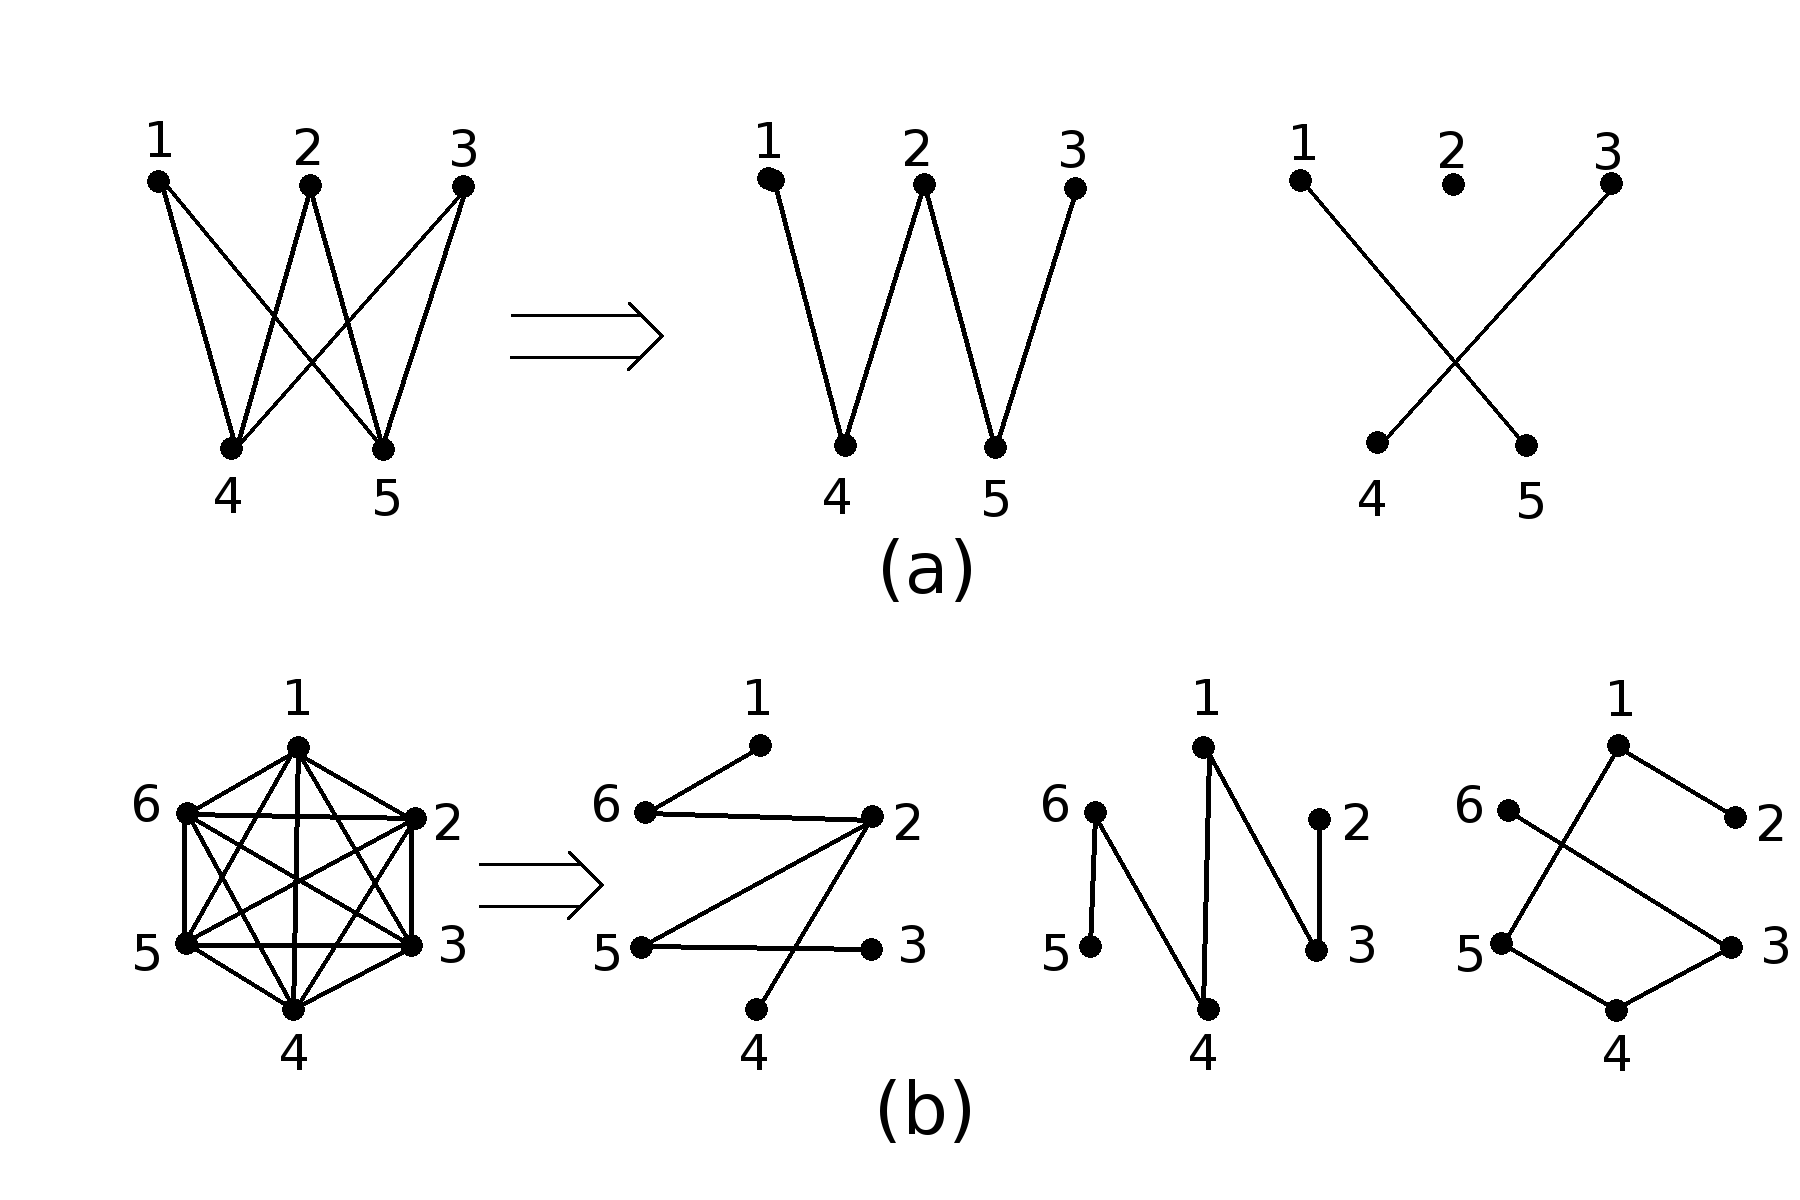
\includegraphics[width=1\textwidth]{images/ceyhun-221-fig01}
		\caption{Ağaç ayrışımı a) İ(2,3) b) D(6). }
	\end{figure}	
\end{document}